
V předchozí kapitole jsme rozebrali veškerý software z Apache Big Data Stacku kromě jednoho. Cassandra je NoSQL WideColumn databáze a jedná se o nejdůležitější software z Apache Big Data Stacku z pohledu této práce, která se právě na Cassandru zaměřuje. Z tohoto důvodu tuto databázi nyní do detailu rozebereme. 

\section{Proč Cassandra}
Přestože NoSQL databází vhodných k uchovávání a zpracovávání BigData existuje celá řada, vybral jsem si Cassandru, protože si myslím, že je nejzajímavější z hlediska architektury. Dosahuje skvělých výsledků v porovnávacích testech\cite{benchmark}, používají ji v produkci a velikých clusterech známé společnosti, má největší komunitu (a na vývoji se aktivně podílejí i velké firmy) a je nejpoužívanější databází ve své kategorii\cite{dbengines}. V neposlední řadě také proto, že jsem se s touto databází setkal již dříve a chtěl jsem zjistit, kam se databáze za tu dobu pohnula.

Díky široké nabídce funkcí a výše popsaným důvodům si myslím, že je tato databáze vhodná i pro edukační účely zejména pro její jednoduchost a zároveň komplexnost. Vzhledem k jednoduchosti začlenění s ostatním softwarem z Apache Big Data Stacku se stává z Cassandry ultimátní BigData nástroj. Absolventům může přijít vhod také fakt, že Cassandra je průmyslově nejpoužívanější databází svého druhu. %citace?


\section{Vznik}

Cassandra vznikla v roce 2008 ve společnosti Facebook, kde sloužila jako úložiště zpráv mezi uživateli této obří sociální sítě. Facebook později téhož roku uvolnil zdrojové kódy projektu. Projekt se v roce 2009 dostal do inkubační fáze pod záštitou Apache Foundation. O rok později – v roce 2010 – se projekt dostal mezi plnohodnotné projekty Apache Foundation. Jak již bylo zmíněno, velké rozdíly mezi verzemi jednotlivých projektů z Apache Big Data Stacku způsobují závažné problémy s kompatibilitou celého systému. Ani Cassandra není výjimkou, i její rozdílné verze nesou rizika a rozdílné funkce a samozřejmě také nekompatibilitu. V současné době je nejaktuálnější verzí Cassandra 2.04 a pokud nebude uvedeno jinak, uvažujeme v textu tuto verzi. 

\section{Předchůdci}

Když Facebook vydal článek popisující Cassandru \cite{facebookcassandra}, popsal ji jako \uv{To nejlepší z Google BigTable a Amazon DynamoDB}, což není náhoda, neboť prvotním šéfem vývoje Cassandry ve Facebooku byl právě inženýr, který ve společnosti Amazon navrhl a vytvořil databázi Dynamo. Podoba s BigTable také není náhodná, Facebook pro své potřeby potřeboval wide-column databázi, a proto byla inspirace BigTable přirozenou volbou. 

\subsection{Co Cassandra zdědila od Dynama}
\begin{itemize}
\item \textbf{Symetrie} Každý uzel má stejnou zodpovědnost a roli v systému.
\item \textbf{Decentralizace} Rozšíření symetrie. Každý uzel může plně komunikovat s jakýmkoliv jiným uzlem a získávat od něj informace. Je tedy možné ovládat systém skrze kterýkoliv uzel, což přispívá k výborným škálovacím vlastnostem. 
\item \textbf{Heterogenita} Každý uzel může mít jiné vlastnosti (např. kapacitu disků) a přidání nového uzlu s jinými vlastnostmi by tím pádem nemělo systém nikterak ohrozit. 
\end{itemize} 

\subsection{Co Cassandra zdědila od BigTable}
\begin{itemize}
\item \textbf{Datový model} Stejně jako BigTable má Cassandra Wide-Column schéma reprezentované klíčem a hodnotou.
\item \textbf{Distribuovaný log} K zápisu používá databáze interně distribuovaný \uv{append log}. 
\end{itemize} 

\section{Kdo Cassandru používá v produkci}

Cassandru v produkčním nasazení můžeme nalézt u mnoha významných společností, které ji používají v clusterech s velikostí od pár uzlů až po největší známý Cassandra cluster o velikosti 400 uzlů a 300 TB dat. Mezi nejznámější společnosti patří:

\begin{itemize}
\item Twitter
\item Ebay
\item Spotify
\item NetFlix
\item Cisco
\item Urban Airship
\item Reddit
\item Accenture
\item a mnoho dalších…
\end{itemize} 

\begin{figure}[h]
\centering

\includegraphics[scale=0.45]{images/casa-production}
\caption{Ukázka ostatních firem využívajících Cassandru v produkčním prostředí}
\label{fig:yarn}
\end{figure}


\section{Společnosti vyvíjející Cassandru}
Cassandra je open source projekt, který je ovšem rozvíjen dvěma velkými společnostmi Acunu a Datastax. Především druhá jmenovaná společnost má na vývoji a budoucnosti Cassandry velkou zásluhu. Datastax pořádá školení a certifikuje vývojáře a administrátory, pořádá setkání a především Cassandru přidává do svého komerčního BigData balíčku, který je nadstavbou Apache Big Data Stacku přidávající vlastní funkcionalitu a spojující všechny komponenty v jeden funkční celek. Pro nekomerční užití v testovacích prostředích je tento balíček k dispozici zdarma.
\section{Hlavní výhody}

Cassandra nabízí pro vývojáře mnoho lákadel. Nyní tu vypíši ty nejzajímavější, které si později rozebereme ve větším detailu. 

\begin{itemize}
\item \textbf{Replikace} Systém sám replikuje data podle kriterií, která mu zadáme.
\item \textbf{Transparentní škálování} Programátor může napsat kód proti lokální instanci a aplikace bude fungovat v jakémkoliv clusteru.
\item \textbf{Nastavitelná konzistence} Můžeme měnit nastavení konzistence přímo za běhu aplikace.
\item \textbf{Nastavitelná síťová strategie} Správce může definovat strategii, podle které systém pozná, do jakého datacentra (případně racku) má uzel zařadit.
\item \textbf{Cassandra Query Language (CQL)} Dotazovací jazyk velmi podobný SQL
\item \textbf{MapReduce} Podpora Hadoop MapReduce
\item \textbf{Databáze nemá \uv{Single Point of Failure}} Díky plně P2P architektuře není databáze náchylná na výpadek jakéhokoliv uzlu.
\item \textbf{Rychlost} Čtení i zápis dosahuje skvělých výsledků \cite{benchmark} a to i při lineárním škálování. 
\end{itemize} 

\begin{figure}[h]
\centering
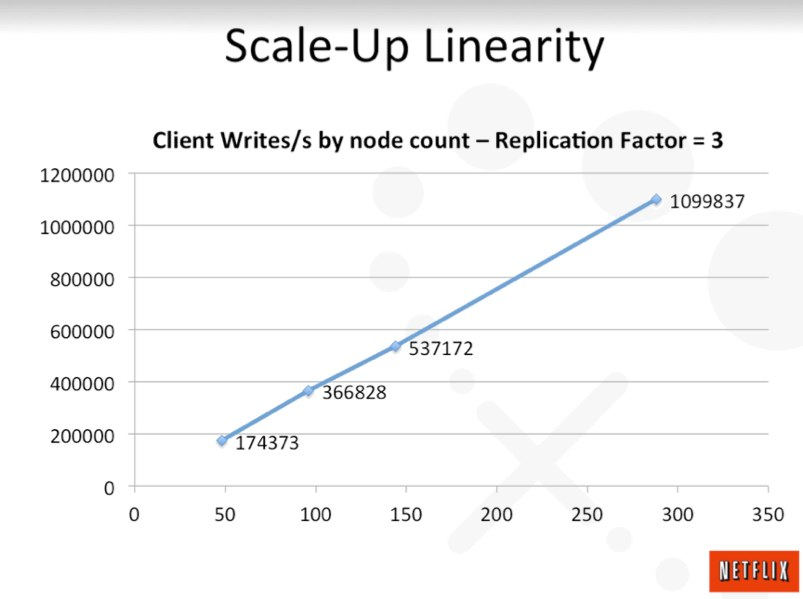
\includegraphics[scale=0.5]{images/netflix}
\caption{Škálování Cassandry a vliv na I/O operace}
\label{fig:scaleup}
\end{figure}

\section{Architektura}
Architektura Cassandry se skládá z několika klíčových bodů, z nichž každý plní svou roli. V následujících podsekcích je stručně vysvětlím.

Cassandra je plně symetrický systém, kde neexistuje jediný bod selhání. Její architektura byla navržena s premisou, že podpůrný hardware a software může padat. Právě proto Casandra nabízí symetrickou architekturu, kde jsou si všechny uzly rovny a veškerá data jsou uložena napříč všemi uzly v clusteru. Commit logy na každém uzlu zachycují veškeré zápisy a data jsou rovněž ukládána do mezipaměti. Když dojde k jejímu zaplnění, tak se data zapíší na disk a automaticky zreplikují a následně rozdistribuují po celém clusteru. 

Klientské požadavky na zápis nebo čtení mohou přijít na kterýkoliv uzel z clusteru a ten se pak pro daný požadavek stává koordinátorem, který se stává jakousi proxy mezi klientem a uzlem, který data vlastní. Tato architektura nám zajišťuje lineární škálování viz \ref{scaleup}

\subsection{P2P protokol \uv{Gossip}}
Do češtiny bychom mohli název tohoto protokolu přeložit jako štěbetání nebo klábosení. Tento název je vlastně velmi trefný, neboť to je v podstatě právě to, co spolu servery dělají. Plně Peer to peer architektura systému s protokolem, kde si jednotlivé uzly o sobě sdělují všechny informace nám dává k dispozici systém, kde každý uzel ví, kde má hledat která data, který uzel je nedostupný, a kterému uzlu by měl nějaká data poslat. Když do systému připojíme nový uzel, ostatní uzly ho ihned začnou zahrnovat informacemi o všech ostatních uzlech v clusteru. To samé platí i pro uzly, které se do clusteru vrátí po nějakém výpadku. Každý uzel o sobě ostatním uzlům posílá informace každou vteřinu. Každý uzel pošle informaci o sobě a ostatních až 3 uzlům najednou a informace sebou nese i časové razítko, aby se předešlé informace mohly přepsat. Tímto způsobem se všechny clustery velice rychle dozví veškeré informace o všech ostatních uzlech v clusteru. 

Pokud je uzel označený jako nefunkční, Cassandra na něj neposílá žádně požadavky. Stejně tak může neposílat požadavky na funkční, ale příliš vytížený uzel pomocí dynamického prohledávání. Zapisování dat, o která uzel přišel po dobu svého výpadku, rozebereme v jedné z dalších sekcí. 

\subsection{Rozdělovač}
Rozdělovače (anglicky \uv{partitioner}) určují, jakým způsobem budou data a jejích repliky rozloženy po clusteru. Jednoduše řečeno, jedná se o hashovací funkci, která vezme klíč, jež chceme ukládat a vrátí nám token, podle kterého určíme, na jaké uzly se má tato hodnota zapsat. Na výběr máme ze 3 možností:

\begin{itemize}
\item \textbf{Murmur3Partitioner} - jedná se o počáteční hodnotu, která rozmisťuje data rovnoměrně po clusteru na základě MurMur3 hashovací funkce.
\item \textbf{RandomPartitioner} - rovnoměrně umisťuje data po clusteru na základě MD5 hashovací funkce (je pomalejší než MurMur3).
\item \textbf{ByteOrderedPartitioner} -  Ukládá data po clusteru na základě lexikálního pořadí bytů. Nedoporučuje se kvůli složitému vyvažování a nerovnoměrné distribuci dat. Jedinou výhodou je sekvenční hledání podobných klíčů.
\end{itemize}

\subsection{Distribuce a replikace dat}
Když si zvolíme vhodný rozdělovač, na základě kterého určujeme, kam příslušný klíč patří, musíme serverům přiřadit určitou výseč klíčů. 

\subsubsection{Kruh}
V Cassandře uzly tvoří takzvaný kruh. Podle počtu uzlů v kruhu se vypočte výseč tokenů, které danému uzlu patří. 

\subsubsection{Virtuální uzly}
Cassandra od verze 1.2 přináší zásadní vylepšení v podobě virtuálních uzlů, kde se každý uzel rozdělí na několik virtuálních (každý dostane svou náhodnou výseč), čímž se rapidně snižuje počet tokenů, které uzlu patří. Virtuální uzly zlehčují a vylepšují v Cassandře hned několik úkonů:

\begin{itemize}
\item Tokeny pro nové uzly se přiřazují náhodně samy a pro nové uzly již tedy není nutné tokeny počítat a přiřazovat manuálně.
\item Oprava mrtvého uzlu je mnohem rychlejší, jelikož se na ní podílí všechny ostatní uzly v clusteru a změny probíhají inkrementálně.
\item Po přidání nového uzlu nemusíme dělat složité převažování clusteru, virtuální uzly se vytvoří rovnoměrně mezi ostatními uzly a vezmou si tak od každého uzlu mnohem menší objem dat.
\item Zlepšuje využití heterogenních strojů v clusteru. Strojům s rozdílnou kapacitou můžeme nastavit rozdílný počet virtuálních uzlů.
\end{itemize}

\begin{figure}[h]
\centering
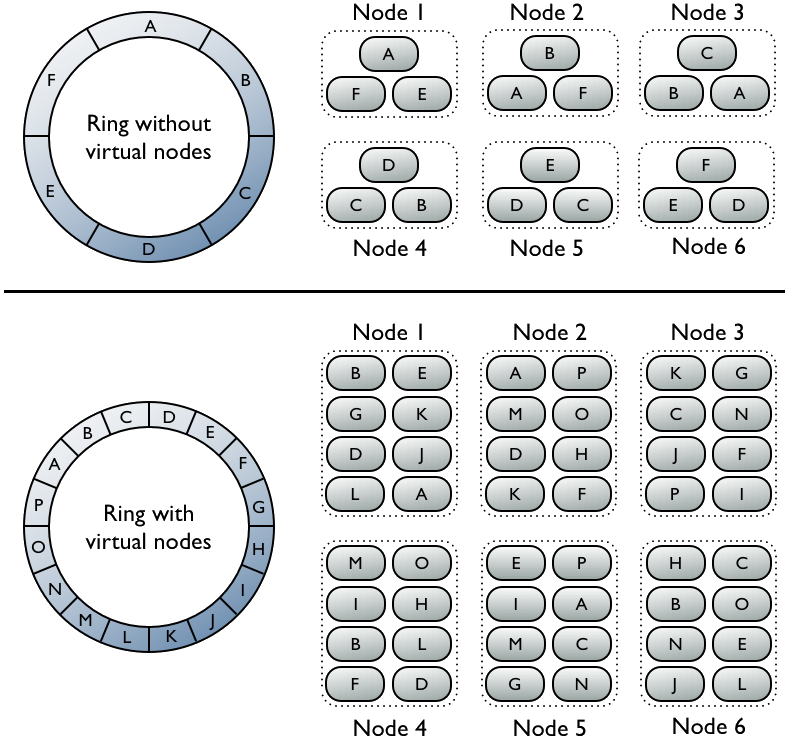
\includegraphics[scale=0.5]{images/vnodes_compare}
\caption{Porovnání uložení dat v kruhu s a bez virtuálních uzlů}
\label{fig:vnodes}
\end{figure}

Když má každý (virtuální) uzel přiřazenu svou množinu tokenů a máme určeno, jak budeme tokeny získávat, je potřeba vyřešit replikování dat. Počet replik je daný replikačním faktorem, který se nastavuje pro každou databázi. Replikační faktor 1 znamená, že každá řádka bude existovat pouze jednou. Replikační faktor 2 znamená, že každá řádka bude uložena dvakrát a pokaždé na jiném stroji. V Cassandře jsou si všechny uzly rovny a to stejné platí také pro repliky dat. Neexistuje tedy žádná hlavní replika, všechny jsou stejně důležité. Replikační faktor by neměl překročit maximální množství uzlů v clusteru, data by pak byla redundantní a ztráceli bysmevýkon. Na výběr máme ze dvou replikačních strategií:


\begin{itemize}
\item \textbf{Jednoduchá strategie} - Využívá se pouze pro clustery uložené v jednom datovém centru. Tato strategie uloží první repliku na uzel určený rozdělovačem a ostatní repliky jsou uloženy na následujících uzlech v kruhu po směru hodinových ručiček bez ohledu na topologii (pozice v racku či datacentru).
\item \textbf{Síťová strategie} - Globální replikační faktor se zde změní na replikační faktor pro každé datacentrum. Každé datacentrum má vlastní kruh. Rozmisťování kopií tedy funguje následovně: První kopie se uloží na uzel vybraný rozdělovačem a další kopie ve stejném datacentru se uloží na nejbližší uzel po směru hodinových ručiček, který se nachází v jiném racku. 
\end{itemize}

\subsection{Donašeči (Snitches)}
Donašeči informují Cassandru o síťové topologii clusteru. Smyslem je, aby požadavky byly směřovány efektivně a aby repliky mohly být uloženy do různých racků či datacenter. 

Na výběr máme několik implementací od jednoduchých, řešících topologii sítě maskováním IP adresy, až po komplexní, kde definujeme topologii ručně. Cassandra nabízí implementace i pro známé cloudové řešení od Amazonu, které dokáže rozeznávat i jednotlivé regiony tohoto poskytovatele.

\subsubsection{Dynamické donášení}
Všechny implementace mají implicitně zapnutou tuto volbu, která se snaží omezit čtení z aktuálně přetížených uzlů směrováním požadavků jinam a chytře tak využívá celý cluster. 

\subsection{Úrovně konzistence}
Cassandra nabízí různé úrovně konzistence pro čtení i zápis. Možné hodnoty a jejich vlastnosti jsou popsané v tabulce \ref{casareads} a tabulce: \ref{casawrites}

\begin{table}
  %  \begin{tabular}{|l|l|}
\begin{tabularx}{\textwidth}{ |l|X| }

    \hline
    Úroveň       & Popis                                                                                                                                                                                                                                                                                  \\ \hline
    ANY          & Zápis se musí provést alespoň na jeden uzel. Pokud jsou všechny uzly, kam má být replika umístěna, nedostupné, můžeme provést zápis do odkladového úložiště. Tyto data však nebudou přístupná ke čtení do té doby, než alespoň jeden uzel vlastnící repliku těchto dat nebude dostupný. \\ \hline
    ONE          & Data musí být zapsána do commit logu a paměti alespoň jednoho uzlu, kde má být replika umístěna                                                                                                                                                                                        \\ \hline
    TWO          & Data musí být zapsána do commit logu a paměti alespoň dvou uzlů, kde má být replika umístěna                                                                                                                                                                                           \\ \hline
    THREE        & Data musí být zapsána do commit logu a paměti alespoň tří uzlů, kde má být replika umístěna                                                                                                                                                                                            \\ \hline
    QUORUM       & Data musí být zapsána do commit logu a paměti na větší polovině uzlů, kde má být replika umístěna                                                                                                                                                                                      \\ \hline
    LOCAL\_QUORUM & Data musí být zapsána do commit logu a paměti na větší polovině uzlů, kde má být replika umístěna v datacentru koordinátorského uzlu.                                                                                                                                                   \\ \hline
    EACH\_QUORUM & Data musí být zapsána do commit logu a paměti na větší polovině uzlů, kde má být replika umístěna v každém datacentru.                                                                                                                                                                  \\ \hline
    ALL          & Data musí být zapsána do commit logu a paměti na všech uzlech, kde má být replika umístěna.                                                                                                                                                                                             \\ \hline
    \end{tabularx}
    \caption {Úrovně konzistence pro zápis}
\label{casawrites}

\end{table}


\begin{table}[!h]
%    \begin{tabular}{|l|l|}
\begin{tabularx}{\textwidth}{ |l|X| }

    \hline
    Úroveň       & Popis                                                                                                                    \\ \hline
    ONE          & Vrátí odpověď z nejbližšího uzlu a na pozadí spustí opravné čtení                                                        \\ \hline
    TWO          & Vrátí aktuální data z dvou nejbližších uzlů (majících repliky)                                                           \\ \hline
    THREE        & Vrátí aktuální data ze tří nejbližších uzlů (majících repliky)                                                           \\ \hline
    QUORUM       & Vrátí nejnovější data poté, co odpoví větší polovina uzlů majících repliky                                               \\ \hline
    LOCAL\_QUORUM & Vrátí nejnovější data poté, co odpoví větší polovina uzlů majících repliky ze stejného datacentra v jakém se nachází koordinátor \\ \hline
    EACH\_QUORUM & Vrátí nejnovější data poté, co odpoví větší polovina uzlů majících repliky z každého datacentra                          \\ \hline
    ALL          & Vrátí nejnovější data poté, co odpoví větší polovina všech uzlů majících repliky                                         \\ \hline
    \end{tabularx}
    \caption {Úrovně konzistence pro čtení}
\label{casareads}

\end{table}


\subsection{Eventuální konzistence}
Cassandra disponuje eventuální konzistencí, což znamená, že úroveň konzistence je proměnlivá. Cassandra tímto obchází zažité paradigma CAP teorému a implementuje tak segmentovanou konzistenci, kterou jsme popisovali dříve. Je na architektovi (a případně vývojáři), kdy jakou úroveň konzistence použije. Cassandra umožňuje zvolit konzistenci pro každý požadavek zvlášť, dokonce i pokaždé jinou pro stejný dotaz. Toto dává architektům a vývojářům obrovskou výhodu při návrhu i samotné implementaci. 

\subsection{Výběr vhodné konzistence}
Univerzální pravidlo pro výběr vhodné úrovně neexistuje, záleží vždy na konkrétní situaci a akci. Obecně ovšem platí, že pokud potřebujeme data rychle, volíme nižší úrovně, naopak pokud vyžadujeme co nejaktuálnější data, použijeme nejvyšší úrovně. 

\section{Klientské dotazy}
Jak bylo zmíněno v předchozích sekcích, Cassandra je plně symetrický systém a tudíž požadavky (jak na čtení, tak zápis) mohou přicházet na kterýkoliv (!) uzel v clusteru. Uzel, který požadavek přijme, se stává koordinátorem a zajišťuje, aby byl úspěšně dokončen. Koordinátor určuje, který uzel vlastní která data na základě rozdělovací a replikační strategie. 

\subsection{Zápis}
Koordinátor pošle požadavek o zápis na \textbf{všechny} uzly, které podle rozdělovací a replikační strategie vlastni tato data. Na tyto uzly budou data zapsána nehledě na úroveň konzistence. Konzistence nám určuje, na kolik odpovědí od uzlů bude koordinátor čekat, než ohlásí požadavek za úspěšný. Úspěšný zápis znamená, že data byla zapsána do commit logu a do mezipaměti. 

Představme si modelovou situaci, kdy máme cluster o 12 uzlech a data zapisujeme s úrovní ONE a replikační faktor máme 3. Koordinátor (v tomto případě uzel 10) pošle požadavek o zápis na uzly 1, 2 a 7. Koordinátor prohlásí požadavek za úspěšný, když mu přijde první odpověď od kteréhokoliv uzlu.

\begin{figure}[h]
\centering
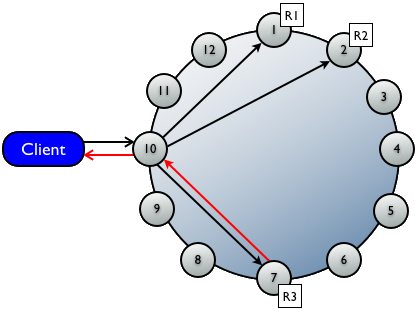
\includegraphics[scale=0.5]{images/write}
\caption{Ukázka zápisu dat s replikačním faktorem 3 a konzistencí 1}
\label{fig:vnodes}
\end{figure}


\subsection{Čtení}
Čtení probíhá dvěma možnými způsoby:

\begin{itemize}
\item Přímé čtení probíhá podobně jako zápis a podrobněji ho rozepíšeme níže.
\item Čtení a opravení dat na pozadí. Jedná se o složitější mechanismus, který popíšeme v následující sekci.
\end{itemize}

Jak již bylo řečeno, přímé čtení funguje podobně jako zápis. Koordinátor odešle požadavek na získání dat všem uzlům, které data vlastní a úroveň konzistence určuje, na kolik správných odpovědí budeme čekat. Data v uzlech mohou být nekonzistentní, Cassandra považuje za správná ta nejnovější data. Konzistenční úroveň u čtení tedy říká, kolik uzlů mi musí vrátit aktuální data. 

V následujícím příkladu uvažujeme stejný cluster jako při zápisu a vyžadujeme data s konzistenční úrovní QUORUM. 2 ze 3 uzlů nám vrátily aktuální data a tedy považujeme celý požadavek za úspěšný. Koordinátor vrátí klientovi data.


\begin{figure}[h]
\centering
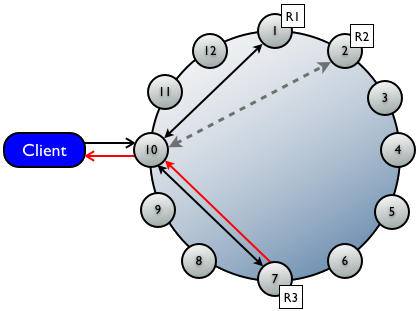
\includegraphics[scale=0.55]{images/read}
\caption{Ukázka čtení dat s replikačním faktorem 3 a konzistencí Quorum}
\label{fig:vnodes}
\end{figure}


\section{Zachování konzistence}%end
Jak bylo naznačeno, při zápisu se může stát, že je uzel nedostupný a nedostane tedy data, která by měl zapsat a tím vznikají nekonzistence dat. Cassandra má 3 interní mechanismy jak si s nekonzistencí dat poradit: 

\begin{itemize}
\item \textbf{Read Repair} Pokud Cassandra při čtení zjistí, že má nějaký uzel nekonzistentní data, pošle po dokončení požadavku na pozadí aktualizační požadavek a data na těchto uzlech aktualizuje. Tato možnost je konfigurovatelná.
\item \textbf{Anti Entropy Node Repair} Pokud byl uzel dlouho nedostupný, můžeme spustit opravný nástroj, který se sám dotáže na konzistenci dat ostatních uzlů a postupně je opraví. 
\item \textbf{Hinted Handoff} Pokud se stane, že je některý z uzlů nedostupný během zápisu, ostatní uzly s replikami si uloží takzvaný hint ohledně zápisu a ve chvíli, kdy se pomocí Gossip protokolu dozví, že daný uzel se vrátil zpět do clusteru, pošlou mu informaci o zápisu. Pokud použijeme při zápisu úroveň konzistence ANY, můžeme zápis provézt úspěšně i pokud budou všechny uzly, kterým data patří, nedostupné. Data a hint se v takovém případě uloží na koordinátorském uzlu. Tato data ovšem nebudou dostupná ke čtení, dokud nebudou řádně zapsána alespoň do jednoho z uzlů kam patří.
\end{itemize}

\section{Oprava dat na disku}
Přestože detailní struktura a ukládání dat na disku je nad rámec tohoto textu, je vhodné říci, že díky své struktuře zděděné od BigTable neprovádí Cassandra žádné inplace úpravy ani mazání. Místo toho používá náhrobky a nové zápisy s aktuálnějšími daty a časovým razítkem. Z toho plyne, že z hlediska zlepšení výkonu a ušetření místa na disku je potřeba čas od času provést pročištění a sjednocení těchto \uv{append-only} souborů. Této technice se říká kompakce a jedná se o pokročilejší administrátorskou úlohu při práci s Cassandrou, která se nachází mimo rámec tohoto textu. %inplace?

\section{Datový model}
Reprezentaci dat a ukládací engine si Cassandra vypůjčila a přizpůsobila od BigTable. Cassandra tedy spadá pod Key-Value storage systémy a WideColumn systémy. Těmto systémům se občas nadlehčeně říka\uv{Fancy hash table}, což můžeme přeložit jako \uv{Honosná HashTabulka}. Důvodem pro toto lehce posměšné označení je jednoduchý princip celého datového modelu, tedy že se jedná \uv{pouze} o ukládání klíče-hodnoty s pár funkcemi navíc. Vzhledem k vyspělosti těchto systémů v dnešní době a rozsáhlosti funkcí, můžeme toto dehonestující označení považovat za pouhý komunitní slovní žert.

Cassandra v dnešní době disponuje moderním rozhraním, které si popíšeme v další sekci. Považuji však za vhodné si připomenout takzvané \uv{legacy API}, které plně odkrývalo reprezentaci dat, jež je důležitá pro pochopení toho, jak vlastně Cassandra funguje uvnitř. V dnešní době je tento engine obalen příjemným SQL-Like rozhraním. Znalosti \uv{legacy API} se nám však mohou hodit při návrhu našeho doménového modelu a optimalizaci dotazů. V neposlední řadě ještě i dnes můžeme použít toto staré Thrift API pro komunikaci s databází. Jak si ale brzy ukážeme, není k tomu žádný rozumný důvod. 

\subsection{Změna myšlení}
Pro uživatele přicházející ze světa relačních databází byl velký problém se vypořádat s úplně jiným přístupem a neubránili se neustálému srovnávání přístupů a pojmů. Pro ovládnutí principů NoSQL (a především efektivního a funkčního návrhu modelů v Cassandře) je důležité myslet na 2 hlavní zásady: 

\begin{itemize}
\item \textbf{Denormalizace} Vše, co jste se učili v SQL systémech o normalizaci dat, zde neplatí. Naopak by takové postupy vedly k nefunkčnímu návrhu. Cassandra neumí JOIN příkazy, které při normalizaci obvykle potřebujete a především NoSQL návrh vyžaduje vzhledem ke své nátuře úplně jiný přístup. 
\item \textbf{Redundance} Tento bod částečně souvisí s normalizací, která nám redundanci dat zakazuje a snaží se jí předejít. Při návrhu NoSQL systémů se držíme paradigmatu, které říká, že redundance dat nevadí, protože cena za mírné navýšení místa na disku je mnohem nižší, než cena za čas a HW potřebný ke spuštění takových dotazů, které by zvládly získat potřebná data bez redundance. Ukládat tedy některá data dvakrát za účelem jejich následného snadného čtení je doporučený postup. 
\end{itemize}

Tento přístup byl pro mnoho vývojářů tězce akceptovatelný a stal se jedním z důvodů, proč Cassandra používá CQL, o kterém si povíme později. I přes všechny její nadstavby je stále užitečné vědět, jak Cassandra funguje interně a navrhovat tak kvalitní datové modely. 

\subsection{základní stavební kameny}
Přestože jsme se chtěli od relačního databázového světa oprostit, pro vysvětlení některých pojmů je nejjednodušší srovnání, a proto v několika následujících bodech přirovnání k relačním databázím využiji.

\begin{itemize}
\item \textbf{Keyspace} - Udržuje pohromadě všechny Column Family a replikační faktor, který se na CF přenáší. Každý Keyspace může mít jiný replikační faktor. Keyspace se dá chápat jako pojem \uv{databáze} z relačního světa. Také má nějaké vlastnosti a ty platí pro všechny Column Families (tabulky), které sdružuje.
\item \textbf{Column Family} - Column Family sdružuje řádky, které obsahují sloupce. V relačním světě bychom mohli CF přirovnat k tabulce, která sdružuje jednotlivé záznamy. 
\item \textbf{Row} - Row je řádka identifikována jednoznačným klíčem (primárním) a obsahuje jednotlivé sloupce s daty. Každá řádka může obsahovat sloupce s odlišnými daty, řádky tedy nemají pevnou strukturu. Řádky bychom mohli přirovnat k jednotlivým záznamům v tabulce relační databáze, ale s tím rozdílem, že řádky v Cassandře nemají pevný formát. 
\item \textbf{Column} - Sloupec je nejmenší a tím pádem finální entitou udržující data v Cassandře. Sloupec má svůj název a hodnotu. Sloupce mají také časové razítko, které určuje čas vložení a dle něj se koordinátoři rozhodují, zda jsou sloupce z různých uzlů aktuální či nikoliv. Cassandra disponuje těmito druhy sloupců:

\begin{itemize}
\item \textbf{Standard} - Standardní obyčejný sloupec, který uchovává jednu hodnotu.
\item \textbf{Composite} - Spojený sloupec se používá, pokud je primární klíč složený z více sloupců. Názvy sloupců v takovém případě obsahují svůj původní název rozšířený o druhou část primárního klíče. 
\item \textbf{Expiring} - Sloupce s omezenou dobou platnosti se hodí, pokud chceme životnost dat omezit nějakou dopředu známou dobou, po kterou jsou data platná. Po vypršení této lhůty jsou data z databáze vymazána.
\item \textbf{Counter} - Čítací sloupce můžeme využít, pokud chceme inkrementálně zvyšovat hodnotu v daném sloupci. Tato metoda se však příliš nepoužívá a raději se data předpočítávají průběžně. 
\end{itemize}
\end{itemize}



Z této architektury lze tedy na první pohled usoudit, že Cassandra je opravdu pouze Key-Value storage systém a modelování komplikovanějších datových modelů je náročnou činností. Velkou výhodou je možnost pojmenování sloupce jakýmkoliv klíčem a tak si i do názvu můžeme zakódovat některé užitečné informace, jako například informaci o pořadí. K datům v této struktuře lze přistupovat pomocí Thrift API, které nám otevírá ukládací datový model Cassandry napřímo a data tak čteme v syrové podobě, tak jak jsou uchována přímo v databázi. Tento postup je však zastaralý a pro komunikaci s databází se doporučuje nástupce tohoto rozhraní, kterým je dotazovací jazyk CQL. 

\begin{figure}[!h]
\centering
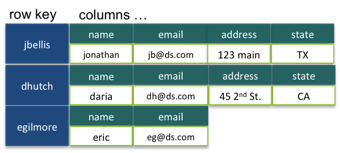
\includegraphics[scale=0.95]{images/static_column_family}
\caption{Schéma datového modelu v Column Family}
\label{fig:vnodes}
\end{figure}

\begin{figure}[!h]
\centering
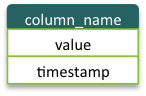
\includegraphics[scale=1.5]{images/column}
\caption{Schéma datového modelu Column}
\label{fig:vnodes}
\end{figure}

\section{CQL}
Přestože bylo v předchozí sekci řečeno, že Thrift je zastaralý a CQL je doporučená cesta jak se dotazovat nad daty, datový model je stále velmi důležitý a je potřeba mu rozumět, abychom dokázali náš model navrhnout funkčně a efektivně. Thrift nám tento model přímo odhaluje a CQL je pouze abstrakcí, která nám dovoluje pracovat s daty obdobně, jako jsme zvyklí v relačním světě s tím rozdílem, že si poté dotazy převede na dotazy nad zmíněným interním datovým modelem. 

CQL je dotazovací jazyk podobný SQL, přes který lze vytvářet datové struktury – tabulky – které mají stejný formát jako tabulky relační, avšak na pozadí se struktury i dotazy nad nimi převedou na datový model popsaný v předchozí kapitole. CQL neumožňuje žádný příkaz z \uv{rodiny} JOIN. Přestože by se mohlo zdát, že pevná struktura nás omezuje oproti předchozím návrhům, opak je pravdou. Pomocí CQL jsme schopni vymodelovat data o různých hodnotách. Konkrétní příklady budou popsány v následující kapitole. 

\newpage

\begin{lstlisting}[caption={Tvorba jednoduché tabulky pomocí CQL},label=CQL1]
CREATE TABLE songs (
  id uuid PRIMARY KEY,
  title text,
  album text,
  artist text,
  data blob
 );
\end{lstlisting}

Jak je z kódu \ref{CQL1} patrné, syntaxe jazyka CQL se opravdu od SQL příliš neliší. Jazyk má různé funkce, ale také určitá omezení, jejichž kompletní popsání by vydalo na samostatnou práci. Jen krátce bych chtěl upozornit, že jazyk podporuje indexy na sloupcích, ale také datové kolekce. Nejdůležitější funkce a omezení budou rozebrány v rámci případů užití v následující kapitole. Na závěr přikládám tabulku převodů interních typů na typy využívané v jazyce CQL.

\begin{table}[h]

    \begin{tabular}{|l|l|l|}
    \hline
    Internal Type     & CQL Name      & Description                                    \\ \hline
    BytesType         & blob          & Arbitrary hexadecimal bytes (no validation)    \\ \hline
    AsciiType         & ascii         & US-ASCII character string                      \\ \hline
    UTF8Type          & text, varchar & UTF-8 encoded string                           \\ \hline
    IntegerType       & varint        & Arbitrary-precision integer                    \\ \hline
    Int32Type         & int           & 4-byte integer                                 \\ \hline
    LongType          & bigint        & 8-byte long                                    \\ \hline
    UUIDType          & uuid          & Type 1 or type 4 UUID                          \\ \hline
    TimeUUIDType      & timeuuid      & Type 1 UUID only (CQL3)                        \\ \hline
    DateType          & timestamp     & Date plus time, encoded as 8 bytes since epoch \\ \hline
    BooleanType       & boolean       & true or false                                  \\ \hline
    FloatType         & float         & 4-byte floating point                          \\ \hline
    DoubleType        & double        & 8-byte floating point                          \\ \hline
    DecimalType       & decimal       & Variable-precision decimal                     \\ \hline
    CounterColumnType & counter       & Distributed counter value (8-byte long)        \\ \hline
    \end{tabular}
    \caption {Interní Datové typy}
   \label{datatypes}
\end{table}